\documentclass[11pt,a4paper]{article}
\usepackage[margin=1in]{geometry}



\usepackage{setspace}
\onehalfspacing
\usepackage{amsmath,amssymb,amsthm,amsfonts}
\usepackage{bm,mathtools}
\usepackage{booktabs,multirow,array,tabularx,caption,subcaption,graphicx,float,xcolor,rotating}
\usepackage{adjustbox}
\usepackage{enumitem}\setlist{nosep,leftmargin=1.5em}
\usepackage[bf,sf]{titlesec}
\titleformat{\section}{\large\bfseries}{\thesection.}{0.6em}{}
\titleformat{\subsection}{\normalsize\bfseries}{\thesubsection}{0.5em}{}
\usepackage[numbers,sort&compress]{natbib}
\bibliographystyle{plainnat}
\usepackage[hidelinks]{hyperref}
\newcommand{\PD}{\ensuremath{\mathrm{PD}}}
\newcommand{\LGD}{\ensuremath{\mathrm{LGD}}}
\newcommand{\EAD}{\ensuremath{\mathrm{EAD}}}
\newcommand{\RWA}{\ensuremath{\mathrm{RWA}}}
\newcommand{\EL}{\ensuremath{\mathrm{EL}}}

\newcommand{\BDT}{\textsc{BDT}}
\newcommand{\EUR}{\textsc{EUR}}
\newcommand{\AUTHORCHECK}[1]{{\color{red}\textbf{[AUTHORS TO CONFIRM: #1]}}}
\captionsetup{font=small,labelfont=bf}
\newcommand{\tabsize}{\footnotesize}

\title{\bfseries From Scores to Capital and Prices:\\
How Calibration, Selection and Regulatory Treatment Move\\
Basel III Outcomes in SME Lending}
\author{Anmita Das\thanks{\texttt{aadas@student.unimelb.edu.au}}
\quad Shoumya Chowdhury\thanks{Corresponding author: \texttt{shoumyac@student.unimelb.edu.au}}\\[2pt]
\small Faculty of Engineering and Information Technology, University of Melbourne, Australia}
\date{}
\begin{document}
\maketitle

\begin{abstract}
\noindent
Credit scoring research is judged on discrimination, yet a probability of default matters economically only after it passes through a non linear regulatory capital formula, a risk based price and an approval rule. We study that passage on 1{,}200 Bangladeshi SME loan applications ({{prev:.2f}}\% twelve month missed payment rate) and replicate the calibration and recalibrator findings on five public credit data sets from five countries (subgroup slope heterogeneity, by contrast, is clearly detectable in the largest of them). Four results stand out. First, calibration is a first order modelling choice. A class balanced logistic score reports a mean default probability of {{raw_mean_pd:.1f}}\% against {{prev:.1f}}\% observed; recalibrating it cuts the Brier score by {{brier_gain_pct:.1f}}\% and raises the share of borrowers priceable under a 22\% rate ceiling from {{cw_bal_via:.1f}}\% to {{cw_pl_via:.1f}}\% (five seed means; unweighted training needs no such correction). Isotonic regression, the usual recommendation, collapses the portfolio onto {{I_distinct:.0f}} probability values, assigns {{iso_floor_pct:.1f}}\% of borrowers a three basis point default probability, and understates Tier 1 capital by {{-t1_iso_vs_platt_pct:.1f}}\%. Second, apparent subgroup calibration disparities are largely sampling noise: after recalibration no subgroup shows significant bias in calibration in the large, the dispersion of subgroup bias and of subgroup discrimination is within what a perfectly calibrated model would produce at these sample sizes, only weak slope heterogeneity (two groups) is detected, and per group recalibration does not pay for its variance. We therefore bound, rather than assume, the capital and price error that undetectable miscalibration could cause (capital between {{bd_cap_lo:.0f}}\% and +{{bd_cap_hi:.0f}}\%, rates between {{bd_rate_lo:.1f}} and +{{bd_rate_hi:.1f}} points). Third, selection matters more than subgroup effects: a model trained on a historically screened sample under predicts default among excluded applicants by {{-sc_cil_max:.0f}} to {{-sc_cil_min:.0f}} points, and inverse propensity reweighting does not repair it. Fourth, regulatory treatment and the definition of default are first order: classifying these exposures as retail rather than corporate SME lowers mean capital by {{-retail_drop_pct:.1f}}\%, and a Basel like default definition (here an illustrative conversion share of one half) moves the priceable share by {{dd05:.1f}} points, so regulatory treatment is larger than the recalibration effect on capital. Risk based pricing under the ceiling turns lending into a screening problem: a flat 18\% rate loses BDT {{flat_loss:.0f}} million on the sample while the screened portfolio earns the hurdle return and its default rate falls from {{prev:.1f}}\% to {{N_pool_default:.1f}}\% (out of fold). The screen, not the price, produces the fall. The screen also reduces approval of rural borrowers to {{rural_app:.0f}}\% against {{urban_app:.0f}}\% for urban ones. In a stylised design, a partial credit guarantee that absorbs only unexpected loss restores BDT {{ul_incr:.0f}} million of credit at no expected fiscal outlay. All inputs, code and tables are reproducible from a single script chain.
\bigskip

\noindent\textbf{Keywords:} credit scoring; probability calibration; Basel III IRB; risk adjusted return on capital; SME finance; selection bias; emerging markets; Bangladesh.
\end{abstract}

\section{Introduction}
Machine learning credit scoring has advanced almost entirely on rank based metrics \citep{Khandani2010,Lessmann2015}. A lender, however, does not use a rank. It uses a probability to set regulatory capital under the Basel III internal ratings based (IRB) approach \citep{BCBS2017}, to price the loan so that the return on that capital clears a hurdle \citep{Repullo2004,Stoughton2007}, and to decide whether the loan is made at all under any binding rate ceiling. The capital formula is non linear in the probability, the price is a function of the capital, and the approval rule is a threshold on the price. Small errors in a probability are therefore not small errors in an outcome.

Two bodies of work say what can go wrong, but they rarely meet. The calibration literature shows that scores are often miscalibrated, that the damage is hardest to see in small subgroups, and that common training devices such as class weighting distort probabilities \citep{Guo2017,VanCalster2019,Roelofs2022,VanDenGoorbergh2022}. The regulatory finance literature shows that capital and price are sensitive to loss given default, correlation and the definition of default \citep{Tarashev2010,Witzany2008,Altman2005}. We connect them: we follow a single probability through the capital formula, the price and the approval decision, and measure how each upstream modelling choice, and each limitation of the data, moves the economic outcome.

\subsection{Setting and data}
We use 1{,}200 SME loan applications from Bangladesh ({{n_def:.0f}} defaults, {{prev:.2f}}\%) and, to test generality, five public credit data sets from Germany, Taiwan, the United States, Poland and Australia. Bangladesh is a useful case because a flat or near flat lending rate is common market practice, a statutory ceiling binds, and credit rationing rather than price dispersion is the realistic outcome \citep{Beck2006,Berger2006}.

\subsection{Contributions}
\begin{enumerate}[label=\textbf{C\arabic*.}]
\item \textbf{From score to capital, price and decision, with uncertainty.} A complete pipeline from a recalibrated probability to the IRB capital requirement, a RAROC consistent rate and an approval decision under a rate ceiling, with bootstrap intervals on every headline quantity (Section~\ref{sec:headline}).
\item \textbf{Calibration as a first order choice.} Class balanced weights give a mean default probability of {{raw_mean_pd:.1f}}\% against {{prev:.1f}}\% observed, which removes {{cw_gap:.0f}} points of priceable share; the granularity of the recalibrator moves capital by {{-t1_iso_vs_platt_pct:.0f}}\% (Section~\ref{sec:prob}).
\item \textbf{An honest power analysis of subgroup calibration.} Bootstrap intervals and a parametric null show that apparent group level calibration disparities are mostly noise at these sample sizes, and we bound the capital and price error that undetectable miscalibration could produce (Section~\ref{sec:subgroup}).
\item \textbf{A selection experiment.} A truncation experiment on labelled data measures the bias a historically screened training sample imparts to the excluded population, and tests a standard repair (Section~\ref{sec:selection}).
\item \textbf{Regulatory treatment, default definition and loss given default.} Retail versus corporate classification and a Basel like default definition move the results by more than the hurdle rate, while collateral linked LGD mainly redistributes access across borrowers (Section~\ref{sec:capital}).
\item \textbf{Screening versus pricing.} We decompose the benefit of risk based pricing under a ceiling into a screening component and a price component, add take up and adverse selection, a downturn, and a thresholded fairness audit (Sections~\ref{sec:regimes} and~\ref{sec:robust}).
\item \textbf{A priced policy remedy.} A partial credit guarantee design that absorbs only unexpected loss (Section~\ref{sec:guarantee}).
\item \textbf{Five country replication.} The calibration, class weighting and recalibrator findings are replicated on five public data sets (Section~\ref{sec:external}).
\end{enumerate}

\subsection{Roadmap}
Section~\ref{sec:related} reviews related work, Section~\ref{sec:data} the data, Section~\ref{sec:method} the methods. Sections~\ref{sec:prob} to~\ref{sec:guarantee} report results, Section~\ref{sec:external} the replication, Section~\ref{sec:disc} discusses what generalises and what remains open, and Section~\ref{sec:conc} concludes.

\section{Related work}\label{sec:related}
\paragraph{Calibration in credit scoring.} Calibration means that predicted probabilities match observed frequencies. Modern classifiers are often miscalibrated \citep{Guo2017}, and post hoc scaling by Platt's logistic method or isotonic regression is the standard remedy \citep{Platt1999,Niculescu2005,ZadroznyElkan2002}. In clinical prediction, calibration has been called the Achilles heel of predictive analytics \citep{VanCalster2019}, and rebalancing the classes to improve ranking is shown to damage calibration \citep{VanDenGoorbergh2022}. Prior shift between a training and a deployment prevalence has a closed form correction \citep{Saerens2002,Elkan2001}. Calibration error estimators are themselves biased in small samples, and detecting miscalibration of ten percentage points in a group of a few hundred observations is difficult \citep{Roelofs2022}. Credit studies that report calibration typically do so pooled; we are not aware of one that reports subgroup calibration with intervals and a sampling null, and then propagates the result to capital.

\paragraph{Fairness and selection.} Group fairness is usually assessed on thresholded decisions \citep{Hardt2016,Kleinberg2017,Chouldechova2017,Pleiss2017}; in credit, \citet{Kozodoi2022} study fairness and profit trade offs. Models are trained on accepted applicants only, so default behaviour of rejected applicants is unobserved, which biases scorecards \citep{BanasikCrook2007}. We measure that bias directly in a controlled truncation experiment.

\paragraph{Capital, pricing and SME lending.} The IRB risk weight function rests on the asymptotic single factor model \citep{Vasicek2002,Gordy2003}; \citet{Tarashev2010} show parameter uncertainty has first order effects and \citet{Witzany2008} study sensitivity to the default definition. Risk adjusted return on capital underpins risk based pricing \citep{Froot1998,Stoughton2007,Saunders2010}, and \citet{Repullo2004} characterise loan prices under capital requirements. \citet{Altman2005} and \citet{Vozzella2020} examine SME capital and regulatory correlations. SMEs in emerging markets face information asymmetry and rationing \citep{Beck2006,Berger2006,Petersen1994,StiglitzWeiss1981}; \citet{Bjorkegren2020} and \citet{Berg2020} study alternative data. The closest study is \citet{Durango2024}, who price microcredit using IRB capital; they do not treat a binding ceiling, regulatory treatment, or recalibration.

\paragraph{Gap.} We know of no study that (i) follows a recalibrated probability through capital, price and approval; (ii) quantifies, with a sampling null, how much subgroup miscalibration matters to capital and price; (iii) measures selection bias on labelled data and its capital consequence; and (iv) replicates the calibration findings across countries.

\section{Data}\label{sec:data}
\subsection{Bangladeshi SME sample}
The sample contains $n={{n:.0f}}$ SME loan applications from 2022 to 2023 with firm and owner characteristics, loan request characteristics, four text fields and a binary outcome recording whether the firm missed any scheduled payment in the following twelve months (prevalence {{prev:.2f}}\%, {{n_def:.0f}} events). Inputs to the capital formula are the disbursed amount (exposure at default, EAD), the requested tenor clipped to one to five years (maturity $M$, which makes the pipeline a foundation LGD, advanced maturity hybrid), and annual sales (twelve times monthly revenue at 100 BDT per Euro, clipped to the regulatory five to fifty million Euro range). The records were obtained from BASIC Bank Limited and Bangladesh Bank for this research, with permission from the Ministry of Finance of Bangladesh, which was shown to the banks before the data were released. All fields, including the four free text description fields and the outcome, were supplied by the banks.

\subsection{External data sets}
To test generality we use five public credit data sets: the German credit data \citep{Hofmann1994} (1{,}000 consumer loans), the Taiwan credit card default data \citep{Yeh2009} (30{,}000), the United States Give Me Some Credit data (150{,}000 borrowers), the Polish companies bankruptcy data (three year horizon, listed firms) and the Australian credit approval data (690). They were retrieved from OpenML and the UCI repository. They differ in borrower type, prevalence and size; they carry no loss given default, and some carry no exposure amount, so we use unit exposure where needed and report capital per unit of exposure. They test calibration and capital mechanics, not the Bangladeshi policy results.

\subsection{Ethics}
Permission for the research was granted by the Ministry of Finance of Bangladesh. The research extract contains no personal identifiers and may be shared publicly. \AUTHORCHECK{add an ethics approval or exemption reference if one exists}

\section{Methodology}\label{sec:method}
\subsection{Probability of default}
Let $y_i\in\{0,1\}$ be the twelve month outcome. A logistic regression on the structured features (ten numeric, nine categorical) with class balanced weights and L2 penalty ($C=1$) is fitted by stratified five fold cross validation (seed 42) and produces an out of fold score $\hat p_i$ \citep{Pedregosa2011}. Class balancing implicitly moves the training prior to one half, so $\hat p_i$ is not a default probability. We compare four ways of using it: the raw score; Platt scaling \citep{Platt1999}, a logistic regression of $y$ on $\mathrm{logit}(\hat p)$; isotonic regression \citep{ZadroznyElkan2002}; and the analytic prior correction $\mathrm{odds}\times\pi/(1-\pi)$ \citep{Saerens2002}. Probabilities are clipped to $[0.0003,0.9999]$. Where the screen must not see its own labels we refit the recalibrator nested within the folds.

\subsection{Calibration and subgroup diagnostics}
We report the Brier score \citep{Brier1950}, log loss, the five bin expected calibration error, the calibration slope and intercept, and calibration in the large (CIL, mean prediction minus observed rate) \citep{Steyerberg2010}. For each of 18 subgroups (four sectors, seven divisions, urban/rural, five education levels; $n$ from 85 to 936) we compute percentile bootstrap intervals (1{,}000 resamples), a $z$ test of CIL under the null that the model is calibrated in the group with Holm correction, and a parametric null: outcomes are redrawn from the model's own probabilities (so the model is perfectly calibrated in every group), and the range across groups of the slope, CIL and AUC is recorded 1{,}000 times. The observed range is compared with that null.

\subsection{Basel III IRB capital}
For borrower $i$ with recalibrated $\PD_i$, annual sales $S_i$ in Euro millions and maturity $M_i$, the SME asset correlation is
\begin{equation}
R_i = 0.12\,w_i + 0.24\,(1-w_i) - 0.04\Bigl(1-\tfrac{S_i-5}{45}\Bigr),\qquad w_i=\tfrac{1-e^{-50\PD_i}}{1-e^{-50}},
\end{equation}
with the maturity adjustment $\mathrm{MA}_i=\frac{1+(M_i-2.5)b_i}{1-1.5b_i}$, $b_i=(0.11852-0.05478\ln\PD_i)^2$, and the capital requirement per unit of exposure
\begin{equation}
K_i=\LGD\Bigl[\Phi\Bigl(\tfrac{\Phi^{-1}(\PD_i)+\sqrt{R_i}\,\Phi^{-1}(0.999)}{\sqrt{1-R_i}}\Bigr)-\PD_i\Bigr]\mathrm{MA}_i .
\end{equation}
Risk weighted assets are $\RWA_i=12.5\,K_i\,\EAD_i$ and Tier 1 capital is $0.06\,\RWA_i$. Because sales are below the Euro 5 million floor for every borrower the firm size term is pinned at its maximum. We also compute the other retail function ($R=0.03w^{r}+0.16(1-w^{r})$ with decay 35 and no maturity adjustment) and the standardised approach.

\subsection{Risk based pricing and the approval rule}
Expected loss is $\EL_i=\PD_i\,\LGD$. The RAROC consistent rate equates the return on capital to a hurdle $h$:
\begin{equation}
r_i = r_f+s_F+c_O+\frac{\EL_i+h\,K_i}{1-\PD_i},
\end{equation}
with $r_f=9\%$, funding spread $s_F=2\%$, operating cost $c_O=3\%$, $h=15\%$, $\LGD=45\%$. A borrower is priceable if $r_i\le\bar r=22\%$. The ceiling is an assumed stylised value between the 2022 to 2023 scheduled bank cap and the Microcredit Regulatory Authority cap \citep{BangladeshBank2024,BangladeshBank2020}; Section~\ref{sec:capital} varies it. Profit per borrower is $[(r_i-r_f-s_F-c_O)(1-\PD_i)-\PD_i\LGD]\EAD_i$. Two regimes are compared: a flat 18\% rate for all, and RAROC pricing for the priceable set.

\subsection{Extensions that address data limitations}
\paragraph{Uncertainty.} Headline quantities are bootstrapped over borrowers with the recalibrator refitted in each resample (1{,}000 resamples).
\paragraph{Selection.} A historical scorecard rank is built from profit to loan ratio, collateral and late payment history. The least attractive $q$ of applicants are treated as historically rejected; the model and its recalibrator are trained on the accepted only and evaluated on the rejected, whose labels we observe. A random exclusion of the same size is the control, and inverse propensity weights (acceptance modelled on observables) are the standard repair.
\paragraph{Take up and adverse selection.} Take up is $1/(1+e^{k(r-0.18)\cdot100})$ and the realised default odds of those who accept rise by $e^{\gamma(r-0.18)\cdot100}$, over $k\in\{0,0.15,0.3\}$ and $\gamma\in\{0,0.03,0.06\}$ per percentage point.
\paragraph{Downturn.} Default odds are scaled by $\{1,1.5,2,3\}$ and LGD raised to 0.55.
\paragraph{Collateral linked LGD.} LGD is 0.60, 0.45 and 0.30 for low, moderate and high collateral (and a steeper scheme).
\paragraph{Thresholded fairness.} Approval rates, approval rates among borrowers who did not default, and the ratio of lowest to highest group approval are computed for each attribute with bootstrap intervals.
\paragraph{Default definition.} The label is any missed payment, wider than the Basel 90 days past due criterion. Let $\phi$ be the share of missed payment events that qualify; the prior shift correction maps $\PD$ to a probability with mean $\phi\bar\pi$.
\paragraph{Reproducibility.} All results come from Python 3 scripts with scikit learn \citep{Pedregosa2011} and fixed seeds; each table in this paper is generated directly from the output files.

\section{Results I: probabilities}\label{sec:prob}
\subsection{Discrimination and the headline numbers}\label{sec:headline}
The pooled out of fold ROC AUC is {{auc_pooled:.3f}} (95\% bootstrap interval {{ci_auc_lo:.3f}} to {{ci_auc_hi:.3f}}). Table~\ref{tab:ci} gives the headline economic quantities with bootstrap intervals. The point estimates are tight enough to support the qualitative claims: the share priceable is between {{ci_v_lo:.0f}}\% and {{ci_v_hi:.0f}}\%, Tier 1 capital between BDT {{ci_t_lo:.0f}} and {{ci_t_hi:.0f}} million, and the flat regime loses between BDT {{ci_f_lo:.0f}} and {{ci_f_hi:.0f}} million.
\begin{table}[H]\centering\tabsize\caption{Headline quantities under Platt recalibration with 95\% bootstrap intervals.}\label{tab:ci}
{{T_ci}}\end{table}

\subsection{Class weighting breaks the probability}
The balanced weight score has a mean of {{raw_mean_pd:.1f}}\% (seed 42; 36.9\% averaged over five seeds) against an observed rate of {{prev:.2f}}\% and a calibration slope of {{slope_pooled:.2f}} with intercept {{int_pooled:.2f}}. Used directly as a probability it makes only {{cw_bal_via:.1f}}\% of borrowers priceable; recalibrated, {{cw_pl_via:.1f}}\%. Table~\ref{tab:cw} repeats this over five seeds and compares unweighted training. Unweighted logistic regression is already close to calibrated on the mean ({{cw_none_raw:.1f}}\%), and the analytic prior correction removes most but not all of the bias (ECE {{cw_ana_ece:.3f}} against {{cw_pl_ece:.3f}} for Platt), because penalised logistic regression shrinks scores. Discrimination is unchanged by weighting. The Brier score of the Platt probabilities is {{brier_gain_pct:.1f}}\% lower than that of the balanced weight score, but about the same as that of an unweighted model; the gain is the removal of a self inflicted distortion. The mechanism is the one in the clinical literature \citep{VanDenGoorbergh2022}; here it shows up in capital and approval.
\begin{table}[H]\centering\tabsize\caption{Class weighting and recalibration, mean of five cross validation seeds (Bangladeshi data).}\label{tab:cw}
{{T_cw}}\end{table}

\subsection{The recalibrator}\label{sec:recal}
Isotonic regression fitted to 1{,}200 observations is a step function. Table~\ref{tab:recal} shows it yields {{I_distinct:.0f}} distinct probabilities, with {{I_at_floor:.0f}} borrowers ({{iso_floor_pct:.1f}}\%) at the three basis point floor, none of whom defaulted, and a Brier score lower than Platt in sample ({{I_brier:.3f}} versus {{P_brier:.3f}}) that is not preserved out of fold ({{NI_brier:.3f}} versus {{N_brier:.3f}}, the same to three decimals). The capital formula inherits the steps: mean $K$ is {{I_mean_K:.2f}}\% against {{P_mean_K:.2f}}\% and total Tier 1 is BDT {{I_total_t1:.0f}} million against {{P_total_t1:.0f}} million. A probability of three basis points is not credible for a borrower population with a quarter defaulting; it is an artefact of the fit. We therefore use Platt scaling as the primary recalibrator and report isotonic results alongside. Figure~\ref{fig:cal} shows the reliability curves and the atoms.
\begin{table}[H]\centering\tabsize\setlength{\tabcolsep}{3pt}\caption{Probability estimates and downstream consequences. ``Nested'' refits the recalibrator on four folds and applies it to the fifth.}\label{tab:recal}
{{T_recal}}\end{table}
\begin{figure}[H]\centering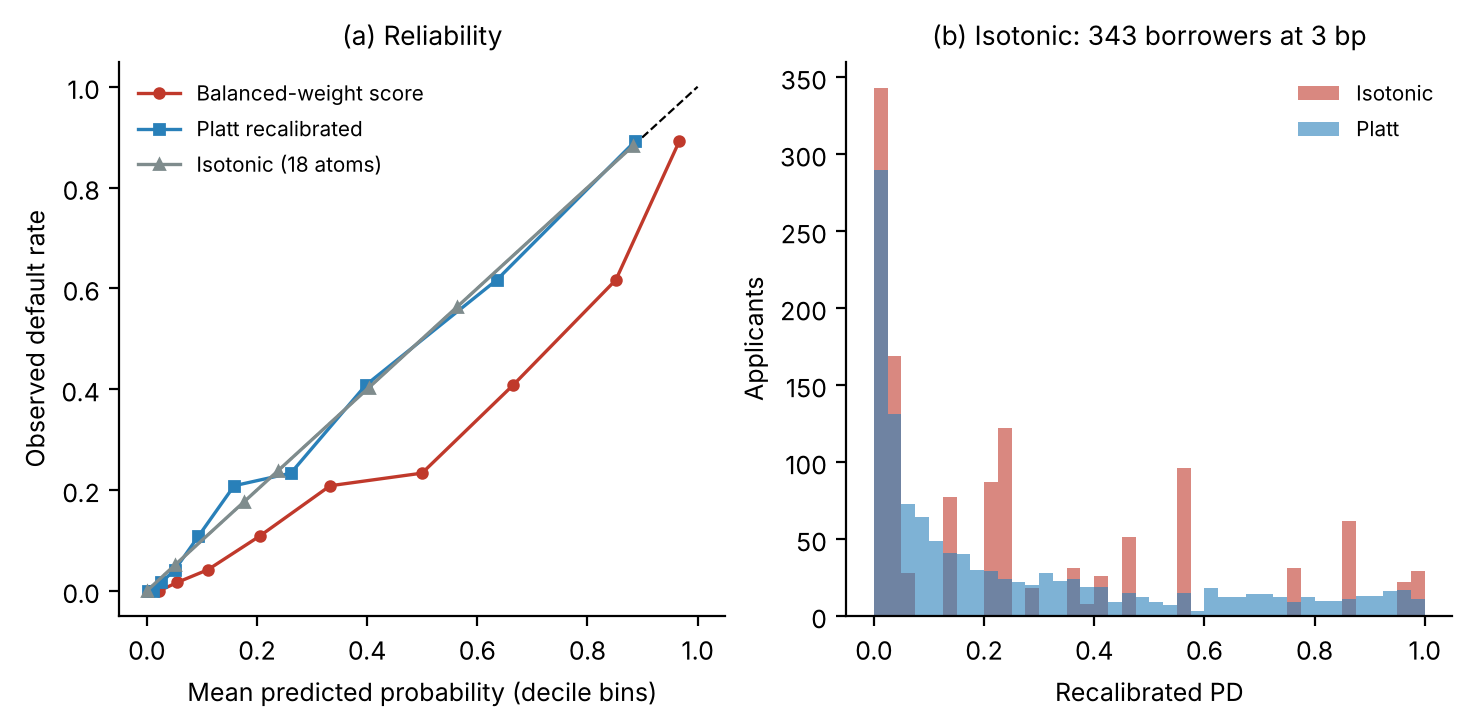
\includegraphics[width=.92\textwidth]{figures/fig1_calibration.png}\caption{(a) Reliability of the balanced score, Platt and isotonic probabilities in decile bins. (b) Distribution of recalibrated PDs.}\label{fig:cal}\end{figure}

\section{Results II: are subgroups miscalibrated?}\label{sec:subgroup}
\subsection{Intervals and a sampling null}
Table~\ref{tab:sub} and Figure~\ref{fig:forest} report calibration and discrimination for the 18 subgroups with bootstrap intervals. For the balanced score every subgroup is significantly over predicted (Holm adjusted, {{raw_sig:.0f}} of 18), by {{raw_cil_min:.1f}} to {{raw_cil_max:.1f}} percentage points; this is the uniform class weighting bias, not a group specific effect. After Platt recalibration {{plat_sig:.0f}} of 18 subgroups differ significantly from calibration in the large.

The dispersion across groups is what a calibrated model would produce by chance. Table~\ref{tab:null} compares observed ranges with the parametric null. The range of subgroup CIL is {{cil_rng_raw:.1f}} points against a null median of {{cil_null_raw:.1f}}; the range of subgroup AUC is {{auc_rng:.3f}} against a null median of {{auc_null:.3f}} ($p={{auc_p:.2f}}$); the range of slopes is {{slope_rng_raw:.2f}} against a null median of {{slope_null_raw:.2f}}, marginally outside the null at the five percent level ($p={{slope_p_raw:.3f}}$ for the balanced score, {{slope_p_p:.3f}} for Platt). The slope signal comes from two groups: Barisal (slope near 1.9 for Platt, interval wide, $n=102$) and higher secondary education owners (slope near 0.77). We read this as weak evidence of slope heterogeneity, not as a calibration disparity between groups. A conclusion that subgroup AUC or calibration ``varies'' on a sample of this size would be an over reading.
\begin{table}[H]\centering\tabsize\setlength{\tabcolsep}{3pt}\caption{Subgroup calibration and discrimination with 95\% bootstrap intervals. CIL is predicted minus observed default rate. Out of fold scores.}\label{tab:sub}
{{T_sub}}\end{table}
\begin{figure}[H]\centering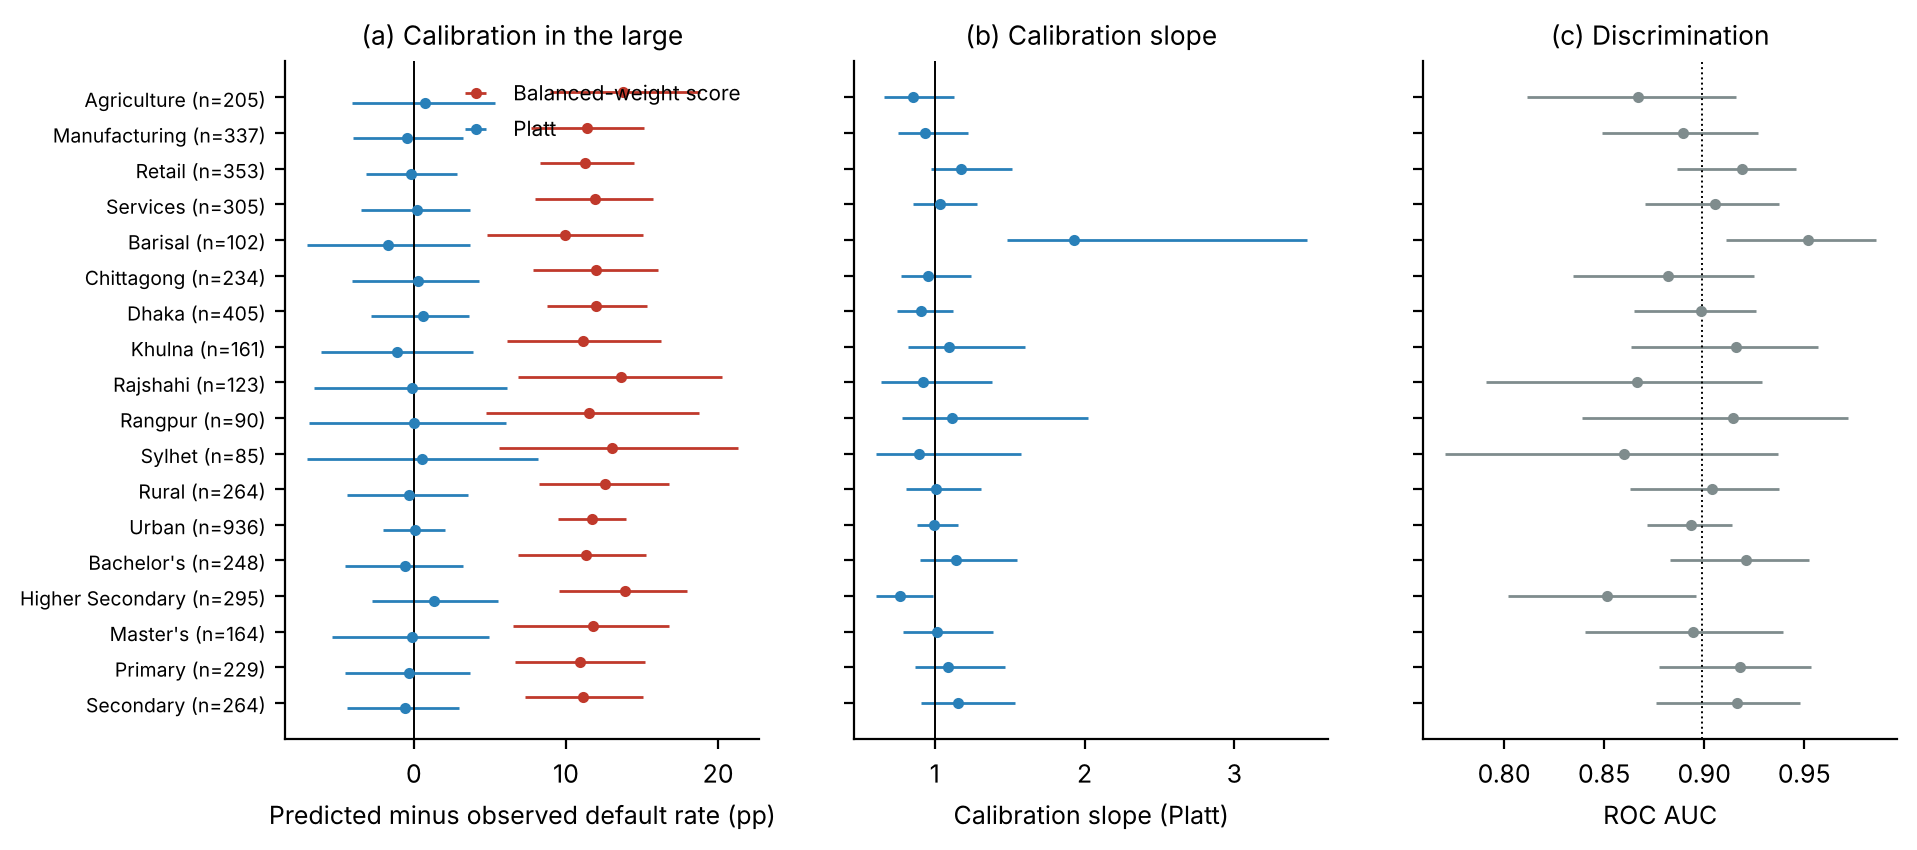
\includegraphics[width=\textwidth]{figures/fig2_subgroup_forest.png}\caption{Subgroup calibration in the large, calibration slope and AUC with bootstrap intervals.}\label{fig:forest}\end{figure}
\begin{table}[H]\centering\tabsize\caption{Observed dispersion across the 18 subgroups versus a perfectly calibrated null (1{,}000 draws).}\label{tab:null}
{{T_null}}\end{table}

\subsection{Does recalibrating per group help?}
Table~\ref{tab:recgrp} compares global Platt and isotonic recalibration with a Platt model that adds group intercepts (unpenalised and shrunk) and with fully group specific Platt models, all cross fitted over ten fold assignments. Group intercepts reduce the largest absolute CIL across groups from 0.3 to 1.6 percentage points under global Platt to 0.1 to 0.3 points, but the pooled Brier score and log loss are slightly worse in every case: the variance cost of estimating group parameters from 85 to 936 observations is not repaid. Per group recalibration is therefore not recommended on these data unless a group is known to differ for a substantive reason.
\begin{table}[H]\centering\tabsize\caption{Cross fitted comparison of recalibrators by attribute (mean of ten fold assignments).}\label{tab:recgrp}
{{T_recgrp}}\end{table}

\subsection{What undetectable miscalibration could cost}
Failing to detect group miscalibration does not prove its absence. We therefore take each group's confidence limits on CIL as the largest plausible hidden error, shift the group's PDs accordingly, and recompute capital and the median rate (Table~\ref{tab:bound}). Hidden errors of the size the data cannot exclude would change group capital by {{bd_cap_lo:.0f}}\% to +{{bd_cap_hi:.0f}}\% and group rates by {{bd_rate_lo:.1f}} to +{{bd_rate_hi:.1f}} percentage points. These bounds are wide because the groups are small, which is the practical meaning of the small subgroup limitation in the literature.
\begin{table}[H]\centering\tabsize\caption{Range across groups of the capital and rate error if the group's PD were mis-stated by the limit of its 95\% interval for CIL.}\label{tab:bound}
{{T_bound}}\end{table}

\section{Results III: selection}\label{sec:selection}
All models in this literature are fitted on borrowers who were accepted. Table~\ref{tab:trunc} and Figure~\ref{fig:trunc} report the truncation experiment. When training excludes applicants by a historical scorecard, the model under predicts default among the excluded by {{-sc_cil_max:.1f}} to {{-sc_cil_min:.1f}} percentage points across the five exclusion shares even though its AUC on them remains {{sc_auc_min:.2f}} to {{sc_auc_max:.2f}}: ranking survives, calibration does not. A random exclusion of the same size leaves bias within {{ra_cil_abs:.1f}} points, so the bias is due to selection rather than to the smaller sample. Inverse propensity weighting based on observables does not help here (bias {{ip_cil_min:.1f}} to {{ip_cil_max:.1f}} points), because the historical rule screens on the very features the propensity model sees and leaves little overlap. The capital consequence is not clear cut: capital is concave in PD, and Tier 1 estimated on the excluded group differs from the full sample reference by a similar amount under random exclusion, so we do not read a capital error from this experiment. The clear consequence is on PD, and hence on the price offered to the riskiest applicants. In practice the through-the-door population is riskier than the booked one and a model trained on bookings will understate its PD; we flag this as a limitation that no analysis without rejected outcomes can remove, and offer the experiment as a way to size it.
\begin{table}[H]\centering\tabsize\setlength{\tabcolsep}{3pt}\caption{Truncation experiment (three of the five exclusion shares shown). Models are trained on accepted applicants and evaluated on the excluded.}\label{tab:trunc}
{{T_trunc}}\end{table}
\begin{figure}[H]\centering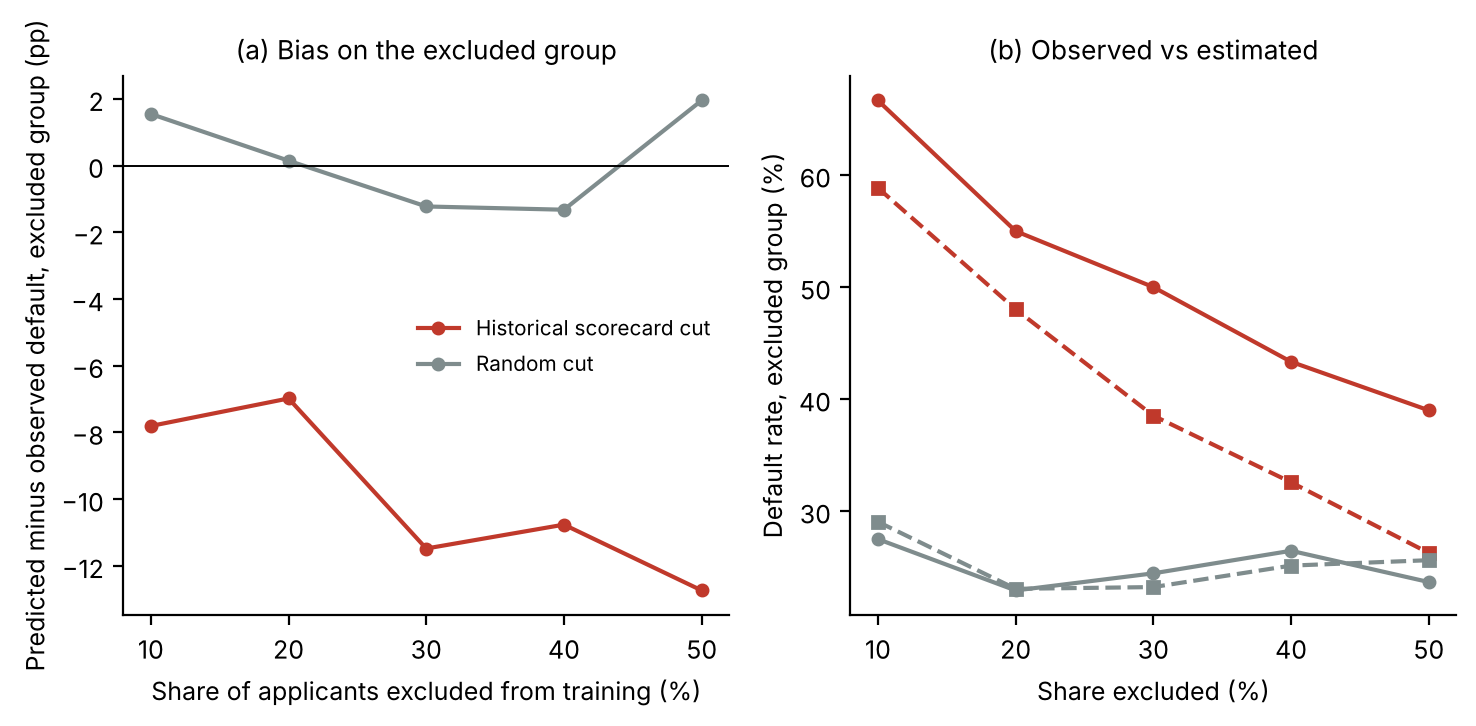
\includegraphics[width=.92\textwidth]{figures/fig6_truncation.png}\caption{Bias on the excluded applicants by the share excluded.}\label{fig:trunc}\end{figure}

\section{Results IV: capital, pricing and regulatory treatment}\label{sec:capital}
\subsection{Capital and prices}
With Platt probabilities the mean capital requirement is {{P_mean_K:.2f}}\% of exposure, mean RWA BDT {{P_mean_rwa_m:.2f}} million, mean Tier 1 BDT {{P_mean_t1_k:.0f}} thousand per applicant and total Tier 1 BDT {{P_total_t1:.0f}} million. The median RAROC rate is {{P_median_rate:.1f}}\% and {{P_viable:.1f}}\% of borrowers are priceable under the 22\% ceiling, representing BDT {{P_credit_m:.0f}} million of credit. Capital peaks and then falls with PD because expected loss is deducted (Figure~\ref{fig:capital}), so the price is far more sensitive to PD than the capital is. Table~\ref{tab:groups} gives results by group: agriculture is the least priceable sector ({{agri_app:.1f}}\% at a median rate of {{agri_rate:.1f}}\%) and rural borrowers have a mean PD of {{rural_pd:.1f}}\% against {{urban_pd:.1f}}\% for urban ones, a median rate of {{rural_rate:.1f}}\% and a priceable share of {{rural_app:.1f}}\% against {{urban_app:.1f}}\%.
\begin{figure}[H]\centering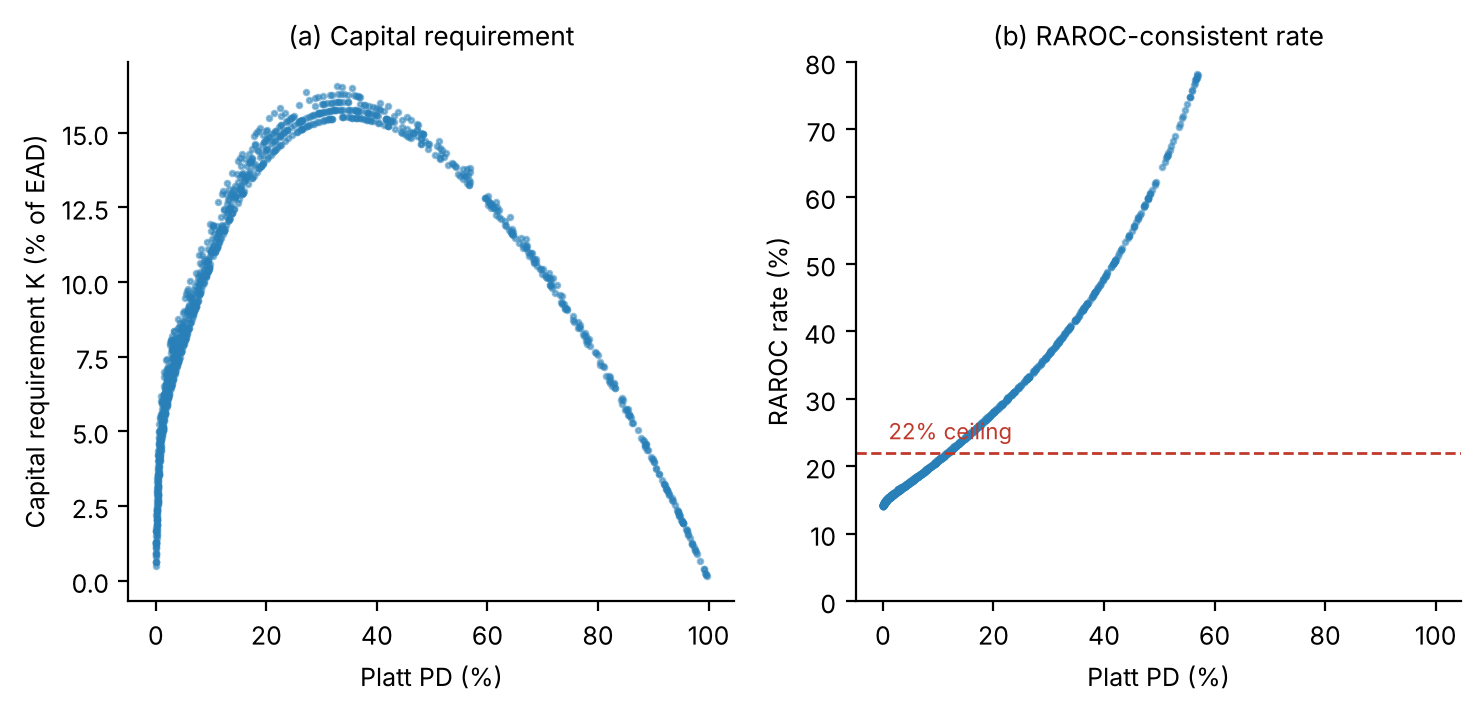
\includegraphics[width=.92\textwidth]{figures/fig3_capital_rate.png}\caption{Capital requirement and RAROC rate against recalibrated PD.}\label{fig:capital}\end{figure}
\begin{table}[H]\centering\tabsize\setlength{\tabcolsep}{3pt}\caption{Capital and pricing by group (Platt PD, corporate SME formula).}\label{tab:groups}
{{T_groups}}\end{table}

\subsection{Sensitivity}
The priceable share is {{P_viable:.1f}}\% in the base case. It rises by {{lgd30:.1f}} points if LGD is 0.30 and falls by {{-lgd60:.1f}} points at 0.60; moving the hurdle to 5\% adds {{h05:.1f}} points and to 25\% removes {{-h25:.1f}} (Table~\ref{tab:sens}, Figure~\ref{fig:sens}). The assumed ceiling matters more than either: at 18\% only {{cap18:.1f}}\% are priceable and at 26\% {{cap26:.1f}}\%. The risk free rate matters too: {{rf7:.1f}}\% at 7\% and {{rf11:.1f}}\% at 11\%.
\begin{table}[H]\centering\tabsize\caption{Share priceable (\%) by LGD and hurdle, and by ceiling and risk free rate (Platt PD).}\label{tab:sens}
{{T_sens}}\vspace{4pt}\\{{T_caprf}}\end{table}
\begin{figure}[H]\centering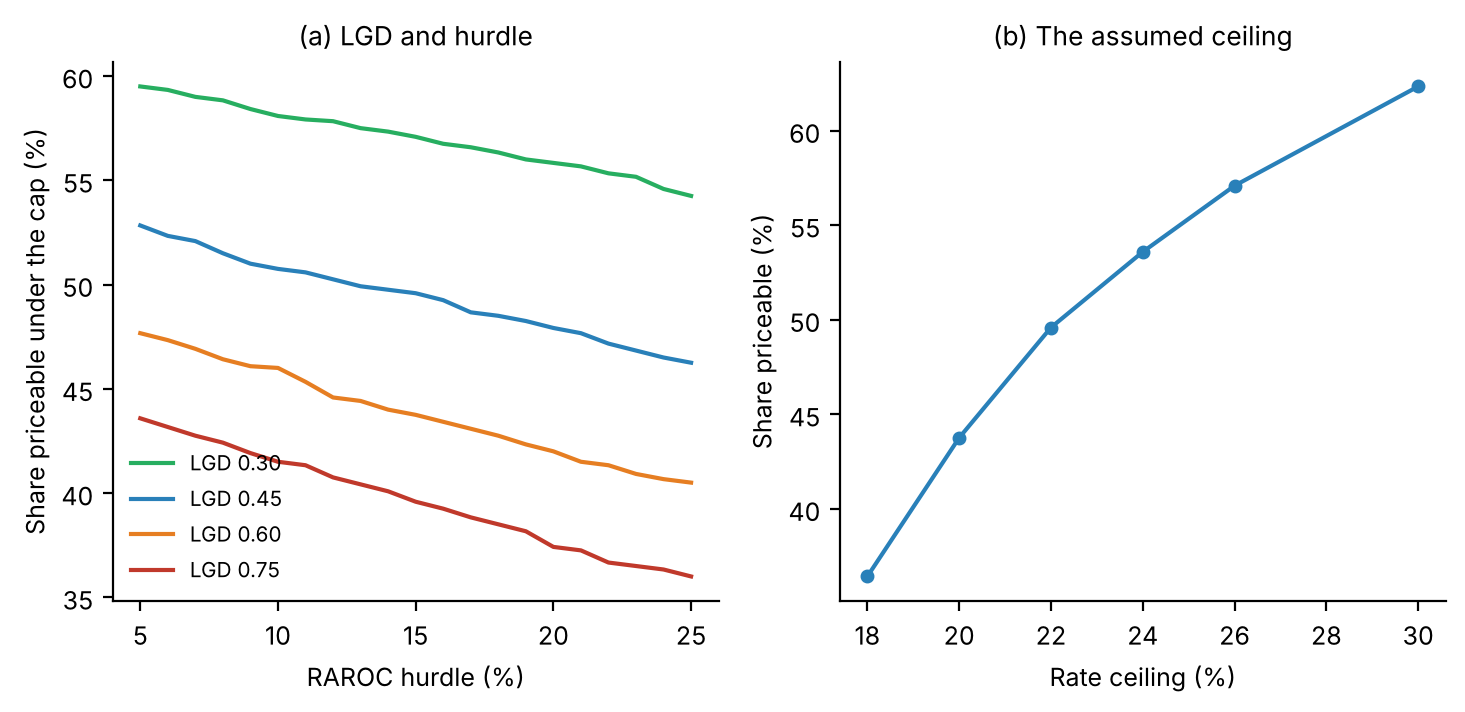
\includegraphics[width=.92\textwidth]{figures/fig4_sensitivity.png}\caption{Sensitivity of the priceable share.}\label{fig:sens}\end{figure}

\subsection{Which Basel treatment applies?}
Every borrower is below the Euro 1 million retail threshold, so on the Basel definitions these are retail exposures. Table~\ref{tab:treat} shows (the isotonic priceable share is unchanged across treatments because it can switch only at one of its 18 atoms) that moving from the corporate SME formula to the other retail formula lowers mean $K$ by {{-retail_drop_pct:.1f}}\% (Platt; {{-retail_drop_pct_iso:.1f}}\% with isotonic) and total Tier 1 from BDT {{P_total_t1:.0f}} to 117 million; the spread across defensible treatments is a factor of {{treat_ratio:.1f}}. The classification therefore matters more than the hurdle rate. Where a regulator or bank can choose among treatments the choice is a capital decision before it is a modelling one.
\begin{table}[H]\centering\tabsize\setlength{\tabcolsep}{3pt}\caption{Regulatory treatment, under isotonic and Platt PD. Tier 1 in BDT million.}\label{tab:treat}
{{T_treat}}\end{table}

\subsection{The definition of default}
The Bangladeshi label is any missed payment; the Basel criterion is 90 days past due or unlikely to pay. With a conversion share $\phi$ of 0.5 the priceable share rises by {{dd05:.1f}} points and Tier 1 falls to BDT {{dd_t05:.0f}} million (Table~\ref{tab:dd}). This lever is larger than doubling the hurdle rate or reducing LGD from 0.45 to 0.30. We do not observe the narrower label, so the table is a sensitivity, not an estimate.
\begin{table}[H]\centering\tabsize\caption{Default definition sensitivity (Platt PD, prior shift correction).}\label{tab:dd}
{{T_dd}}\end{table}

\subsection{Collateral linked loss given default}
The foundation LGD of 0.45 ignores collateral, yet default rates differ ({{lgd_low_def:.1f}}\% for low collateral against {{lgd_mod_def:.1f}}\% moderate and {{lgd_hi_def:.1f}}\% high). Linking LGD to collateral (0.60, 0.45, 0.30) leaves the portfolio total almost unchanged (priceable {{lgd_all_v:.1f}}\%, Tier 1 BDT {{lgd_all_t:.0f}} million) but redistributes it sharply: {{lgd_low_v:.1f}}\% of low collateral borrowers are priceable against {{lgd_hi_v:.1f}}\% of high collateral borrowers (Table~\ref{tab:lgd}). Realised recoveries are not observed in these data, so this too is a sensitivity.
\begin{table}[H]\centering\tabsize\setlength{\tabcolsep}{3pt}\caption{Collateral linked LGD (Platt PD).}\label{tab:lgd}
{{T_lgd}}\end{table}

\section{Results V: pricing regimes}\label{sec:regimes}
Table~\ref{tab:regime} compares the flat 18\% regime with RAROC pricing. The flat regime lends to everyone and loses BDT {{flat_loss:.0f}} million once expected loss is netted. RAROC pricing, applied only to the priceable set, earns BDT {{raroc_profit:.1f}} million (the hurdle return on capital) and lowers the default rate in the pool to {{P_pool_default:.2f}}\% in sample (95\% interval {{ci_pool_lo:.1f}} to {{ci_pool_hi:.1f}}\%) and {{N_pool_default:.2f}}\% with nested recalibration.

The decomposition in the last two rows is informative. Holding the nested screen fixed and charging the flat 18\% instead of the RAROC price leaves approval and default unchanged and gives a higher profit of BDT {{flat_vs_screen:.1f}} million against {{screen_profit:.1f}} million, because the screened pool is safe enough that 18\% over earns relative to the RAROC rate. The fall in default is therefore entirely a property of the screen; the contribution of price differentiation is distributional, lower rates for the safest borrowers and higher rates for the marginal, and it costs the lender margin. Reporting the fall in default as a benefit of risk based pricing would mislead.
\begin{table}[H]\centering\tabsize\setlength{\tabcolsep}{3pt}\caption{Pricing regimes (Platt PD).}\label{tab:regime}
{{T_regime}}\end{table}

\section{Results VI: robustness to what we cannot observe}\label{sec:robust}
\subsection{Take up and adverse selection}
The counterfactual so far holds the pool fixed. Table~\ref{tab:take} lets take up fall with the rate and the accepted pool become riskier with the rate. The flat regime loses the same BDT {{-flat_tk:.0f}} million in every case by construction (at 18\% take up is one half and the adverse selection factor is one); the informative result is that RAROC profit stays positive, between BDT {{tk_lo:.1f}} and {{tk_hi:.1f}} million, for every demand and adverse selection setting, though the simple demand curve is an assumption.
\begin{table}[H]\centering\tabsize\caption{Take up and adverse selection (Platt PD).}\label{tab:take}
{{T_take}}\end{table}

\subsection{A downturn}
Table~\ref{tab:down} scales default odds and LGD. Doubling default odds cuts the priceable share from {{P_viable:.1f}}\% to {{dn_v2:.1f}}\% and the median rate rises sharply, but total Tier 1 moves little (BDT {{dn_t1:.0f}} to {{dn_t2:.0f}} million) because capital is concave in PD beyond a point. LGD at 0.55 raises Tier 1 to BDT {{dn_lgd_t:.0f}} million. The static model understates procyclicality of access rather than of capital, which is the Stiglitz and Weiss channel under a ceiling and complements the capital procyclicality literature \citep{Repullo2014,Behn2016,Gordy2010}.
\begin{table}[H]\centering\tabsize\caption{Downturn scenarios (Platt PD).}\label{tab:down}
{{T_down}}\end{table}

\subsection{Thresholded fairness}
Calibration and AUC by group say little about decisions. Table~\ref{tab:fair} audits approval. The urban rural gap in approval is {{rural_gap:.1f}} points (interval {{rural_lo:.1f}} to {{rural_hi:.1f}}); the ratio of rural to urban approval is {{rural_ratio:.2f}} ({{rural_r_lo:.2f}} to {{rural_r_hi:.2f}}), with a point estimate below the 0.8 benchmark used in disparate impact practice although the interval spans it, and among borrowers who did not default the gap persists but only just excludes zero. The gap tracks the PD difference ({{rural_pd:.1f}}\% against {{urban_pd:.1f}}\%), not miscalibration, which means a calibrated, accurate model still concentrates rationing on rural lending when a ceiling binds. Whether that is acceptable is a policy question; the guarantee below is one remedy.
\begin{table}[H]\centering\tabsize\caption{Approval gaps under the RAROC screen with 95\% bootstrap intervals. Impact ratio is lowest over highest group approval.}\label{tab:fair}
{{T_fair}}\end{table}

\section{A priced policy remedy: partial credit guarantees}\label{sec:guarantee}
Table~\ref{tab:guar} and Figure~\ref{fig:guar} price two designs. In the first a guarantee covers a share of loss, lowering effective LGD; each unit of expected outlay unlocks {{leverage_lo:.1f}} to {{leverage_hi:.1f}} units of additional credit. In the second the guarantee absorbs only unexpected loss, so the lender prices expected loss alone and holds no capital against the exposure. The priceable share becomes {{ul_viable:.1f}}\% and incremental credit BDT {{ul_incr:.0f}} million, at zero expected fiscal outlay (the guarantor pays only in the tail). The second design is a stylised bound; it assumes the guarantor can bear tail risk at no premium and that moral hazard is absent.
\begin{table}[H]\centering\tabsize\setlength{\tabcolsep}{3pt}\caption{Guarantee designs (Platt PD).}\label{tab:guar}
{{T_guar}}\end{table}
\begin{figure}[H]\centering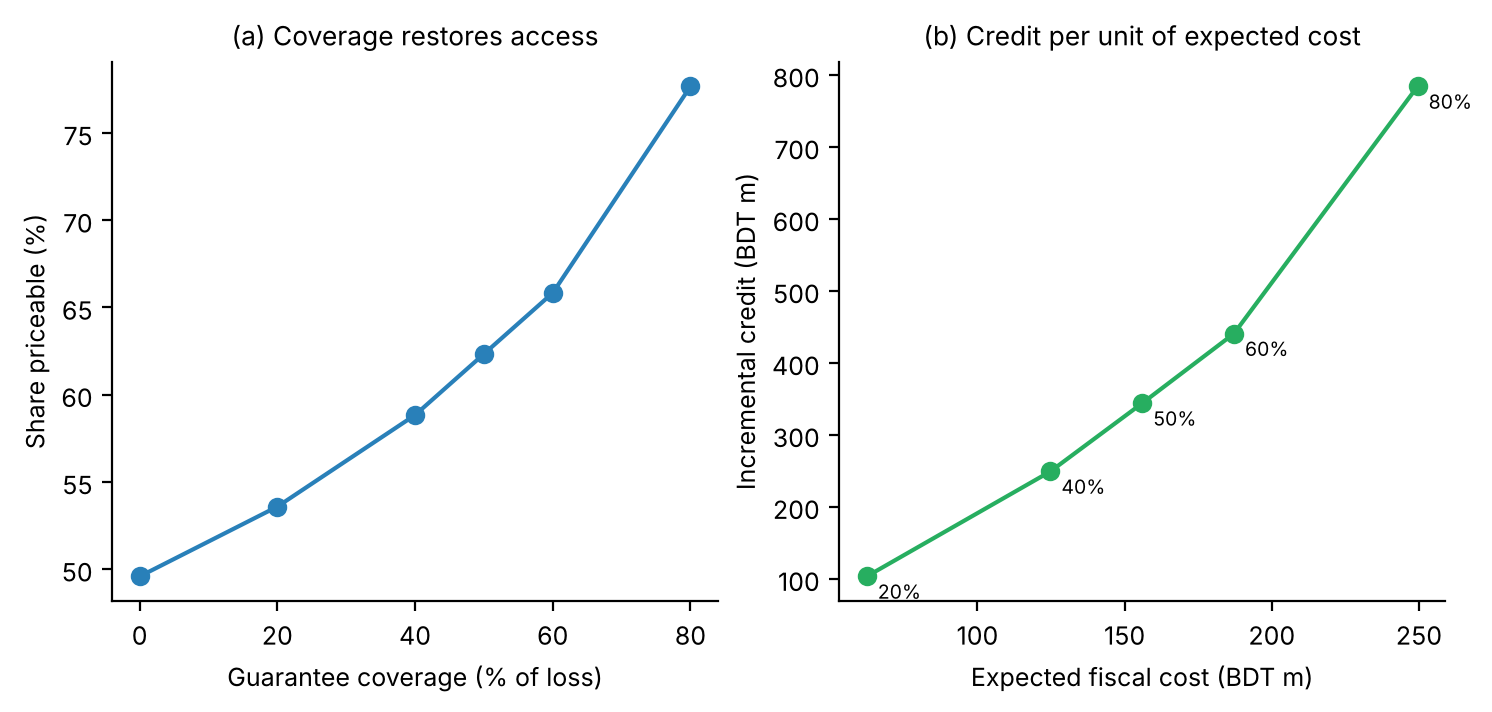
\includegraphics[width=.92\textwidth]{figures/fig5_guarantee.png}\caption{Access and credit under guarantees.}\label{fig:guar}\end{figure}

\section{Replication on five public data sets}\label{sec:external}
Table~\ref{tab:ext} applies the same pipeline (balanced weight logistic regression, five fold out of fold, Platt and isotonic recalibration, IRB capital with the other retail function for consumers and the corporate function for firms, unit exposure, same cost parameters) to five data sets. The balanced weight score overstates mean default by a factor of {{ext_over_min:.1f}} (Australia, where the classes are nearly balanced) to {{ext_over_max:.1f}} (Poland, where defaults are {{ext_pol:.1f}}\% of firms), so the distortion scales with class imbalance; Platt recalibration lowers the Brier score by {{ext_bg_min:.0f}} to {{ext_bg_max:.0f}}\%. The priceable share collapses when the raw score is used as a probability whenever the data are imbalanced. The isotonic artefact depends on sample size: with Taiwan data subsampled to 500 borrowers there are {{tw_atoms_500:.0f}} atoms against {{tw_atoms_30k:.0f}} at 30{,}000, and the priceable share under isotonic is {{tw_viab_iso_500:.0f}}\% against {{tw_viab_pl_500:.0f}}\% under Platt (Table~\ref{tab:isn}, Figure~\ref{fig:isn}). Where subgroup attributes exist the dispersion of calibration across groups is again compared with a perfectly calibrated null (Table~\ref{tab:extnull}). Dispersion of calibration in the large is within noise in all three, but with 150{,}000 borrowers the dispersion of calibration slopes across age bands is clearly real (range {{us_slope:.2f}} against a null 95th percentile of {{us_null:.2f}}). Subgroup slope heterogeneity is therefore detectable when samples are large and cannot be excluded at the Bangladeshi sample size. These data are not SME loans and have no loss given default, so we draw conclusions only about calibration and capital mechanics.
\begin{table}[H]\centering\tabsize\setlength{\tabcolsep}{2.5pt}\caption{Replication across five countries. ``Balanced'' and ``Unweighted'' refer to the training weights.}\label{tab:ext}
{{T_ext}}\end{table}
\begin{table}[H]\centering\tabsize\caption{Isotonic atoms and capital in the replication data sets (balanced weights).}\label{tab:ext2}
{{T_ext2}}\end{table}
\begin{table}[H]\centering\tabsize\caption{Isotonic recalibration against sample size (Taiwan data, ten subsamples per size).}\label{tab:isn}
{{T_isn}}\end{table}
\begin{figure}[H]\centering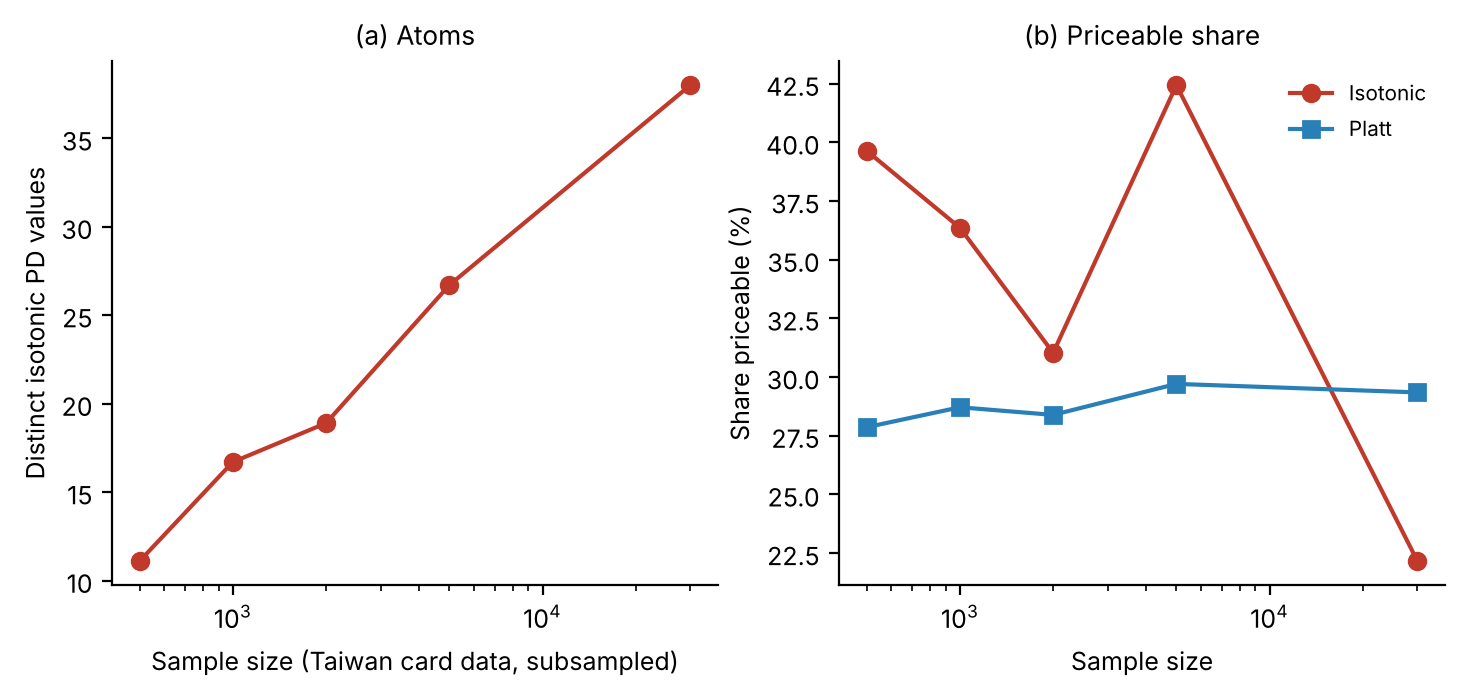
\includegraphics[width=.92\textwidth]{figures/fig7_isotonic_n.png}\caption{The isotonic artefact shrinks with sample size.}\label{fig:isn}\end{figure}
\begin{table}[H]\centering\tabsize\caption{Subgroup dispersion against a calibrated null in the replication data sets.}\label{tab:extnull}
{{T_extnull}}\end{table}

\section{Discussion}\label{sec:disc}
\paragraph{What generalises.} The calibration findings replicate across five countries: class balanced scores are not probabilities, and a step function recalibrator on small samples produces atoms that the capital formula amplifies. The priority is to report calibration, the recalibrator and its granularity whenever a probability enters a non linear formula. The Bangladesh specific policy results (rationing under a ceiling, rural approval, guarantees) generalise to the extent that a rate ceiling binds elsewhere.

\paragraph{What does not survive.} A natural claim, that machine learning credit models are miscalibrated across demographic groups and that this drives unfair pricing, is not supported by the Bangladeshi data. The pooled miscalibration is uniform and removed by one recalibration, and group dispersion is within sampling noise. This is a statement about power as much as about the model: in the 150{,}000 borrower United States sample slope heterogeneity across age bands is clearly present. Group differences in approval arise from group differences in risk. Reviewers should be wary of subgroup calibration claims drawn from samples of a few hundred.

\paragraph{Selection.} Selection is the larger threat. The truncation experiment shows that a model trained on screened applicants will under predict risk for the applicants it has never seen, with ranking intact. A lender extending credit to a wider population, for example through a guarantee, should treat its PD as a lower bound.

\paragraph{Policy.} Under a binding ceiling pricing becomes screening. The default rate improvement comes from refusing loans, not from charging for risk, and its distributional cost falls on rural and agricultural borrowers. Policy makers can address this through ceilings, treatment of exposures as retail, and guarantees, each of which we price.

\paragraph{Limitations.} (i) The Bangladeshi data are a single sample of 1{,}200 with an outcome that is wider than the Basel default; provenance is described in Section~\ref{sec:data}. (ii) LGD is assumed, not estimated; recoveries are unobserved. (iii) The cost of funds, the hurdle and the ceiling are stylised. (iv) There are no rejected applicant outcomes, so selection is sized by experiment, not corrected. (v) Take up, adverse selection and downturn use simple parametric forms. (vi) Fairness is audited on approval, not on welfare or on protected attributes beyond those recorded. (vii) The replication data sets are not SME loans. (viii) The analysis is static; there is no vintage or panel dimension. (ix) Explainability, covered in companion work \citep{Companion2026,CompanionFed2026}, is out of scope.

\section{Conclusion}\label{sec:conc}
A probability of default has economic content only after it passes through capital, price and a decision. On Bangladeshi SME data and five public data sets, calibration is the dominant modelling choice, the recalibrator's granularity matters, subgroup miscalibration is mostly noise at feasible sample sizes but can be bounded, selection bias is the more serious data limitation, and regulatory treatment and default definition move capital by amounts comparable to or larger than the hurdle. Under a binding ceiling risk based pricing is a screen, and its distributional costs can be priced and partly offset by a guarantee.

\section*{Declaration on generative AI}
Generative AI tools were used for coding assistance, language editing and analysis scripting. All research design, interpretation and conclusions are the authors', and the authors take full responsibility for the content.

\section*{Data and code availability}
The Bangladeshi data, all code, every result file and the manuscript source are available at \url{https://github.com/shoumyac/sme-credit-risk-capital-pricing}. The five replication data sets are public (OpenML and the UCI repository) and are downloaded by the replication script.

\bibliography{references}
\end{document}
